\documentclass[tikz,border=5pt]{standalone}
\usepackage{amsmath,amssymb,mathtools}
\usepackage{braket}
\usepackage{xcolor}
\usepackage{tikz}
\usetikzlibrary{arrows.meta,decorations.pathmorphing,decorations.pathreplacing,calc,positioning}

\definecolor{cobalt}{HTML}{2b4c7e}
\definecolor{boxblue}{HTML}{eef3fa}
\definecolor{boxgold}{HTML}{fbf3e3}
\definecolor{boxred}{HTML}{fbecec}
\definecolor{boxgreen}{HTML}{eaf6f0}
\definecolor{ruleblue}{HTML}{2b6cb0}
\definecolor{rulegold}{HTML}{b7791f}
\definecolor{rulered}{HTML}{c0392b}
\definecolor{rulegreen}{HTML}{1f8a5f}

\newcommand{\HH}{\mathcal{H}}
\newcommand{\M}{\mathcal{M}}
\newcommand{\tr}{\operatorname{tr}}
\newcommand{\Tr}{\operatorname{Tr}}
\newcommand{\ii}{\mathrm{i}}
\begin{document}
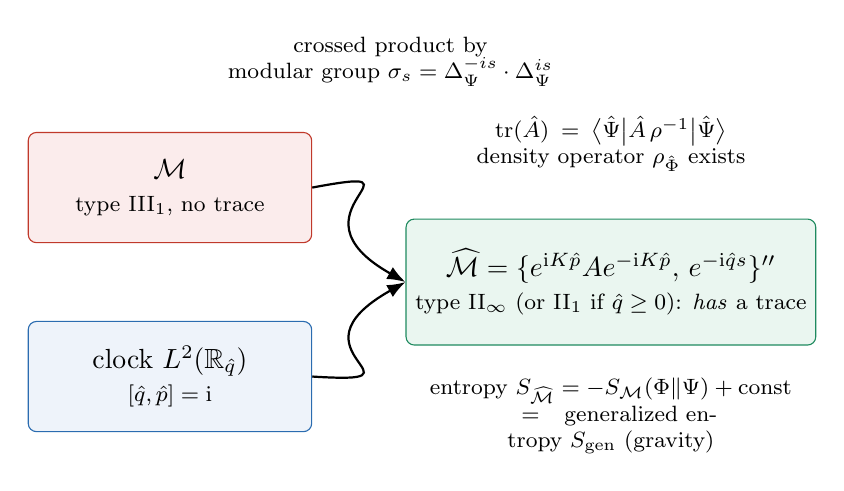
\begin{tikzpicture}[>=Latex, node distance=1.1cm]
\node[draw, rounded corners=3pt, fill=boxred, draw=rulered, align=center, minimum width=3.6cm, minimum height=1.4cm] (M) at (0,0)
  {$\M$ \\ \footnotesize type III$_1$, no trace};
\node[draw, rounded corners=3pt, fill=boxblue, draw=ruleblue, align=center, minimum width=3.6cm, minimum height=1.4cm] (clock) at (0,-2.4)
  {clock $L^2(\mathbb R_{\hat q})$ \\ \footnotesize $[\hat q,\hat p]=\ii$};
\node[draw, rounded corners=3pt, fill=boxgreen, draw=rulegreen, align=center, minimum width=5.2cm, minimum height=1.6cm] (Mhat) at (5.6,-1.2)
  {$\widehat\M=\{e^{\ii K\hat p}Ae^{-\ii K\hat p},\, e^{-\ii \hat q s}\}''$ \\ \footnotesize type II$_\infty$ (or II$_1$ if $\hat q\ge0$): \emph{has} a trace};
\draw[->, thick] (M.east) .. controls +(1.6,0.3) and +(-1.6,0.9) .. (Mhat.west);
\draw[->, thick] (clock.east) .. controls +(1.6,-0.1) and +(-1.6,-0.9) .. (Mhat.west);
\node[align=center, font=\footnotesize] at (2.8,1.6) {crossed product by\\ modular group $\sigma_s=\Delta_\Psi^{-is}\cdot\Delta_\Psi^{is}$};
\node[align=center, font=\footnotesize, text width=3.9cm] at (5.6,0.55) {$\tr(\hat A)=\big\langle\hat\Psi\big|\hat A\,\rho^{-1}\big|\hat\Psi\big\rangle$\\ density operator $\rho_{\hat\Phi}$ exists};
\node[align=center, font=\footnotesize, text width=4.6cm] at (5.6,-2.9) {entropy $S_{\widehat\M}=-S_\M(\Phi\|\Psi)+\text{const}$\\ $\;=\;$ generalized entropy $S_{\rm gen}$ (gravity)};
\end{tikzpicture}

\end{document}
